\documentclass[12pt,a4paper]{report}
\usepackage[utf8]{inputenc}
\usepackage[english]{babel}
\usepackage{amsmath}
\usepackage{amsfonts}
\usepackage{amssymb}
\usepackage{graphicx}

\usepackage{varwidth}

\usepackage{tikz}
\usetikzlibrary{arrows,automata, positioning,calc,shapes.geometric}


\begin{document}


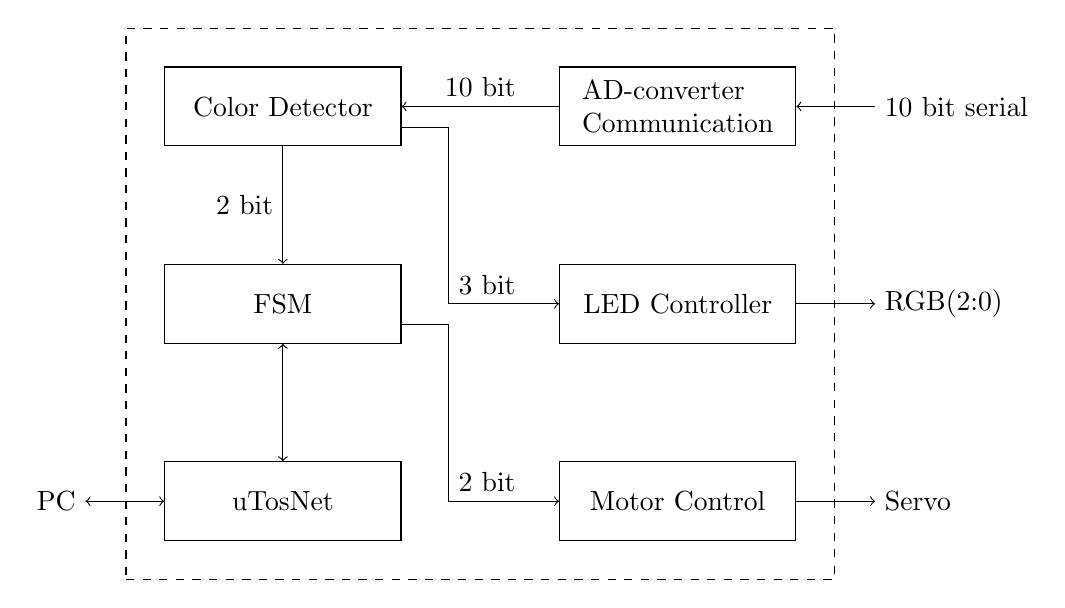
\begin{tikzpicture}[node distance=1cm]



% FPGA border
\node[rectangle,draw,minimum width=9cm, minimum height=7cm, dashed, name=FPGA]  {};

% used to align the insides of FPGA
\node[rectangle,minimum width=5cm, minimum height=5cm, name=FPGAaligne] {};

% components of FPGA
\node[rectangle,draw,minimum width=3cm, minimum height=1cm, name=utos] at (FPGAaligne.-135) {uTosNet};
\node[rectangle,draw,minimum width=3cm, minimum height=1cm, name=ad] at (FPGAaligne.45) {\begin{varwidth}{4cm}AD-converter\\ Communication\end{varwidth}};
\node[rectangle,draw,minimum width=3cm, minimum height=1cm, name=led] at (FPGAaligne.0) {LED Controller};
\node[rectangle,draw,minimum width=3cm, minimum height=1cm, name=mc] at (FPGAaligne.-45) {Motor Control};
\node[rectangle,draw,minimum width=3cm, minimum height=1cm, name=fsm] at (FPGAaligne.180) {FSM};
\node[rectangle,draw,minimum width=3cm, minimum height=1cm, name=color] at (FPGAaligne.135) {Color Detector};

% nodes outside FPGA
\node [left=of utos,name=pc] {PC};
\node [right=of ad,name=adc] {10 bit serial};
\node [right=of led,name=rgb] {RGB(2:0)};
\node [right=of mc,name=servo] {Servo};

% arrows inside FPGA
\draw[<->] (utos) -- node[] {} (fsm) ;
\draw[->] (color.-10) -- ++(0.6,0) |- node[above right] {3 bit} (led) ;
\draw[<-] (color) -- node[above] {10 bit} (ad) ;
\draw[->] (fsm.-10) -- ++(0.6,0) |- node[above right] {2 bit} (mc) ;
\draw[->] (color) -- node[left] {2 bit} (fsm) ;
 
% arrows connected to the outside of FPGA
\draw[<->] (utos) to[out=180, in=0] node[] {} (pc) ;
\draw[->] (adc) to[out=180, in=0] node[] {} (ad) ;
\draw[->] (led) to[out=0, in=180] node[] {} (rgb) ;
\draw[->] (mc) to[out=0, in=180] node[] {} (servo) ;
 
\end{tikzpicture}


\end{document}